\documentclass[a4paper, 12pt]{report}


\usepackage[french]{babel}
\usepackage[utf8]{inputenc}
\usepackage[T1]{fontenc}
\usepackage{lmodern} % load a font with all the characters
%%%%%%%%%%%%%%%%%%%%%%%%%%%%%%%%%%%%%%%%%%%%%%%%%%%%%%%%%%%


\usepackage{amssymb}
\usepackage{setspace}
\usepackage{geometry}

\usepackage{graphicx}     % for images and graphics


\usepackage{subeqnarray}
\usepackage{subfigure}
\usepackage{listings}
\usepackage{color}
\usepackage{caption}
\usepackage{float}

\usepackage{lettrine}
\usepackage{fourier}

\usepackage[pdftex,linkcolor=test,citecolor=vertsombre,colorlinks=true,bookmarks=true, plainpages=true,urlcolor=freeblue]{hyperref}

\usepackage{pdfpages}
\usepackage{fancyhdr}

\usepackage[table]{xcolor}
\usepackage{tabularx}
\usepackage{tabu}


\usepackage{wrapfig}
\usepackage{titlesec}
\setcounter{secnumdepth}{4}
\setcounter{tocdepth}{3}
\makeatletter
\newcounter {subsubsubsection}[subsubsection]
\renewcommand\thesubsubsubsection{\thesubsubsection .\@alph\c@subsubsubsection}
\newcommand\subsubsubsection{\@startsection{subsubsubsection}{4}{\z@}%
                                     {-3.25ex\@plus -1ex \@minus -.2ex}%
                                     {1.5ex \@plus .2ex}%
                                     {\normalfont\normalsize\bfseries}}
\newcommand*\l@subsubsubsection{\@dottedtocline{3}{10.0em}{4.1em}}
\newcommand*{\subsubsubsectionmark}[1]{}
\makeatother

\usepackage[backend=biber]{biblatex}
\addbibresource{biblio/ref.bib}
 
%%%%%%%%%%%%%%%%%%%%%%%%%%%%%%%%%%%%%%%%%%%%%%%%%%%%%%%%%%%
%%%%%     Couleurs      %%%%%%%%%%%
%%%%%%%%%%%%%%%%%%%%%%%%%%%%%%%%%%%%%%%%%%%%%%%%%%%%%%%%%%%

\definecolor{test}{rgb}{0.64,0.16,0.16}
\definecolor{vertsombre}{rgb}{0.00,0.57,0.1}
\definecolor{freeblue}{rgb}{0.25,0.41,0.88}
\definecolor{mygreen}{rgb}{0,0.6,0}
\definecolor{gray}{rgb}{0.5,0.5,0.5}
\definecolor{mymauve}{rgb}{0.22,0.06,0.16}
\definecolor{backcolor}{rgb}{0.95,0.95,0.92}
\definecolor{tabHead}{HTML}{918F90}
\definecolor{tabOdd}{HTML}{EEEEEE}
\definecolor{tabEven}{HTML}{CCCCCC}
\definecolor{codegreen}{rgb}{0,0.6,0}
\definecolor{codegray}{rgb}{0.5,0.5,0.5}
\definecolor{codepurple}{rgb}{0.58,0,0.82}
\definecolor{backcolour}{rgb}{0.95,0.95,0.92}




% \DeclareCaptionFormat{listing}{#1#2#3}
% \captionsetup[lstlisting]{format=listing,singlelinecheck=false, margin=0pt, font={sf}}


\lstdefinestyle{customc}{
  backgroundcolor=\color{backcolour},   
  commentstyle=\color{codegreen},
  keywordstyle=\color{magenta},
numberstyle=\tiny\color{codegray},
    stringstyle=\color{codepurple},
    basicstyle=\footnotesize,
    breakatwhitespace=false,         
    breaklines=true,                 
    captionpos=b,                    
    keepspaces=true,                 
    numbers=left,                    
    numbersep=5pt,                  
    showspaces=false,                
    showstringspaces=false,
    showtabs=false,
    language=bash,
    tabsize=2
}
\lstset{style=customc}


\pagestyle{fancy}
\fancyhf{}
\lhead{\leftmark}
\rfoot{Page \thepage}


\geometry{
left=30mm,
right=20mm,
top=35mm,
bottom=40mm,
headheight=17pt,
}


%An initial of the very first character of the content

\newcommand*{\initial}[1]
{
  \lettrine[lines=3, lhang=0.26, nindent=0em, findent=-1em]
  {
    \color{gray}{\textsc{#1}}
  }{}
}

\newcommand{\clearemptydoublepage}{\newpage{\thispagestyle{empty}\cleardoublepage}}
\newcommand{\clearemptypage}{\newpage{\thispagestyle{empty}}}

\renewcommand{\lstlistingname}{Script}% Listing -> Algorithm


\usepackage[acronym, toc]{glossaries}

\makeglossaries


\newacronym{yaml}{YAML}{YAML Ain't Markup Language}
\newacronym{api}{API}{Application Programming Interface}
\newacronym{iaas}{IaaS}{Infrasturcture As a Service}
\newacronym{paas}{IaaS}{Platform As a Service}
\newacronym{saas}{IaaS}{Software As a Service}
\newacronym{cpu}{CPU}{Central processing unit}

\begin{document}
{\fontfamily{lmr}\selectfont




\includepdf[pages={1}]{cover/cover.pdf}

% \newpage
% \thispagestyle{empty}
% \begin{figure}
% \centering
% 
\includegraphics[trim = 0mm 0mm 0mm 150mm,width=0.7\linewidth]{frontmatter/assets/quran}\\
% 
\includegraphics[trim = 0mm 30mm 0mm 0mm,width=0.65\linewidth]{frontmatter/assets/aya}
% \end{figure}
% \clearemptydoublepage

% \chapter*{Dédicace}
\begin{large}
\begin{center}
\centering

\noindent\textit{
À mes très chers parents 
\newline
Pour votre amour, vos encouragements, vos sacrifices et vos prières 
\newline
Aucun mot ne saura exprimer mes sentiments d’amour, de respect et de gratitude envers vous ; 
\newline
À mes chers frères et sœurs 
\newline
Pour tout ce que vous avez fait pour moi, Je vous souhaite une vie pleine de 
\newline
bonheur et de succès ; 
\newline
À mes chers cousins 
\newline
Pour votre soutien, vos encouragements et votre confiance en moi ; 
\newline
À mes chères amies 
\newline
Pour votre gentillesse, votre compréhension, pour les beaux moments qu’on a passé ensemble, ...bref pour votre amitié ; 
\newline
À toute ma grande famille ; 
\newline
À mon binôme Anas ; 
\newline
À toute personne qui m’est chère ; 
\newline
À tous ceux qui m’aiment ; 
\newline
À tous les musulmans ; 
\newline
À ALLAH avant tout. 
\newline
\newline
\textbf{Un grand Merci à vous.}
\newline
}
\newline
\raggedleft\textbf{\textcolor{white}{text}}
\hfill \textbf{Mohammed}
\end{center}
\end{large}
\clearpage
% \thispagestyle{plain}
\begin{large}
\begin{center}
\centering

\noindent\textit{
    \textbf{À mes très chers parents}
    \newline
    Aucune dédicace ne saurait exprimer l’amour, l’estime, le dévouement et le
    respect que j’ai pour vous.
    \newline
    Rien au monde ne vaut les efforts fournis jour et nuit pour mon éducation et
    mon bien être.
    \newline
    Ce travail est le fruit de vos sacrifices que vous avez consentis pour mon éducation et
    ma formation.
    \newline
    \newline
    \textbf{À mes frères Hamza et Yasser}
    \newline
    \textbf{À ma sœurs Meryem}
    \newline
    Vous étiez toujours sûrs de ma réussite et j’en suis fière.
    \newline
    Vous avez participé dans mon succès par vos encouragements.
    \newline
    « Je vous aime très fort »
    \newline
    \newline
    \textbf{À mes chers tantes, oncles et toute ma grande famille}
    \newline
    Pour votre gentillesse, votre soutien, vos encouragements et votre confiance en moi
    \newline
    \newline
    \textbf{À mes chers amis}
    \newline
    J’ai passé avec vous les meilleurs moments de ma vie, je vous aime
    \newline
    \newline
    \textbf{À mon binôme Mohammed}
    \newline
    Je suis heureux de t’avoir eu comme ami et binôme.
    \newline
}
\newline
\raggedleft\textbf{\textcolor{white}{text}}
\hfill \textbf{Anas}
\end{center}
\end{large}
% \chapter*{Remerciements}
\begin{onehalfspace}
Au terme de ce travail, nous tenons à exprimer notre profonde gratitude et nos sincères remerciements pour tous ceux qui nous ont aidés de près ou de loin pendant la durée de notre stage.
\newline
\newline
Nous tenons également à remercier Monsieur DOUKKALI, professeur à l’ENSIAS pour ses conseils avisés, son encadrement tout au long de ces quatre mois. Nos sincères remerciements sont à adresser à M. OUHAMMI Mohamed et M. ACHARGUI Aminerrahmane qui nous ont fait l'honneur de nous encadrer tout au long de ce travail. Nous leurs en sommes très reconnaissants pour ses fructueux conseils et précieuses directives, et pour le grand souci qu’ils portent à l’égard de notre sujet. 
\newline
\newline
Remerciements spéciaux à tout le corps professoral de l’ENSIAS, pour la formation de qualité qu’ils nous ont prodiguée durant ces trois années. Que tous ceux et celles qui ont contribué de près ou de loin à l’accomplissement de ce travail trouvent l’expression de nos remerciements les plus chaleureux.
\end{onehalfspace}


\chapter*{Résumé}
\begin{onehalfspace}
\initial {L}e présent rapport constitue le fruit d'un travail de trois mois, réalisé dans le cadre de notre projet de fin d'études, et effectué au sein de Sayoo. Le projet a pour objectif de metre en place une architecture Cloud basée sur les conteneurs
\newline
\newline
Il s'agit en effet d'étudier, de concevoir et de déployer une architecture qui va permettre la gestion automatisée des SaaS . Pour arriver à cette fin, nous avons pour mission de développer trois modules essentiels pour tout développement future:

    \begin{itemize}
        \item Le module annuaire.
        \item Le module calendrier.
        \item Le module produit.
    \end{itemize}

\noindent Pour bien mener ce projet, et étant donnée son volet technologique important, nous avons choisit de suivre la démarche de conduite de projet , une démarche qui a fait ses preuves dans le domaine des projets informatiques.
\newline
\newline
Durant ce projet, nous avions pour mission dans un premier temps de cerner le sujet, étudier sa faisabilité et définir le cahier des charges, ainsi que rédiger le dossier de spécifications fonctionnelles aussi bien que technique. Ensuite nous avons entamé l'analyse approfondie et la conception de notre projet, nous avons par la suite élaboré les différents diagrammes , à savoir les diagrammes des cas d'utilisation, les diagrammes de séquences puis les diagrammes de classes, et finalement nous avons passé à l'implémentation, le test et le déploiement de l'application.
\vfill{\textbf{Mots clés:} Cloud, Conteneur, Docker, PaaS, SaaS, Odoo, Deis.}
\end{onehalfspace}

\chapter*{Abstract}
\addcontentsline{toc}{chapter}{Abstract}

\begin{singlespace}
\initial {T}his submission is the result of our work at \emph{Sayoo}, conducted as part of our graduation project. The purpose of our project is to develop a container-based cloud architecture. 
\newline
\newline
In fact, this project aims to reach an architecture that will enable automated management of the company's service. Then, our mission is to study the latest Cloud technologies to get a better knowledge of further parts.
\noindent In order to have a clear view of this project, we've defined several concepts and aspects of the Cloud and its technologies.
\newline
\newline
Initially in this project, we had to identify the issue then define the functional and technical specifications. After, we've focused on the analysis and design parts. We've developed several intermediate architectures that finally lead us to the appropriate architecture.
\vfill{\textbf{Mots clés:} Cloud, Cluster, Scalability, Container, Docker, PaaS, SaaS, Odoo, Deis.}
\end{singlespace}

\cleardoublepage
% \phantomsection Uncomment the \phantomsection line if you're using hyperref
\addcontentsline{toc}{chapter}{\listfigurename}
\listoffigures

\tableofcontents

\chapter*{Introduction}
\addcontentsline{toc}{chapter}{Introduction}

\begin{onehalfspace}
Toutes les entreprises vendent des produits et/ou des services à des clients, évidemment avec l’objectif de générer un chiffre d’affaires et des bénéfices les plus élevés possibles. Le concept du crm est une réponse aux limites du modèle de marketing transactionnel, trop centré sur l’achat et la vente mais ne permettant pas un suivi sur le long terme. Ce concept vise à suivre et à faire évoluer la relation avec le client dans le temps, l’objectif de cette relation étant principalement de fidéliser les clients existants ou de cultiver un vivier de prospects.
\newline
Dans cette optique, la société Thinline a décidé de s’investir dans le développement d'un crm pharmaceutique. Cette plate-forme a pour objectif de faciliter, auprès des laboratoires pharmaceutiques au niveau méditerrané, le suivi et l'évolution de leurs relation avec leurs clients, en automatisant plusieurs processus métier. Dans ce cadre, notre stage de fin d'étude a donc pour objectif de mettre en œuvre cette solution à travers l’étude, la conception et la réalisation de trois modules fondamentaux, à savoir, le module « annuaire», le module « calendrier» et le module « produit».
\newline
Le présent mémoire expose les résultats de notre travail durant notre stage. Il comporte cinq chapitres organisés suivant le processus de développement choisi:
\begin{itemize}
\item L’objet du premier chapitre est de cerner le projet dans son contexte général, à travers la présentation de la société Thinline, pour décrire ensuite la motivation du projet et les objectifs visés. La dernière section du chapitre sera consacrée à la conduite et la planification du projet.
\item Le deuxième chapitre et le troisième chapitre englobent respectivement l’analyse et la spécification des besoins, à savoir l'étude fonctionnelle, dont l’objectif est de capturer les besoins fonctionnels et opérationnels du système futur, aussi bien que l'étude technique, qui englobe l’architecture physique et logicielle ainsi que les outils les plus appropriés pour ce type d'application.
\item Au niveau du quatrième chapitre, nous explicitons les phases d’analyse et de conception de la plateforme. Nous utilisons les différents diagrammes uml pour modéliser les fonctionnalités de l’application.
\item Le cinquième et dernier chapitre décrit d’une façon détaillée, la phase de mise en œuvre du projet, à travers quelques interfaces réalisées.
\end{itemize}

\noindent Le mémoire se termine par une conclusion générale qui présente le bilan du travail réalisé et ses principales perceptives.





\clearpage

\end{onehalfspace}


\chapter{Contexte général du projet}
\begin{onehalfspace}

\initial{L} e présent chapitre permet de situer le projet dans son contexte général, à travers, dans un premier temps, la présentation de l'organisme d'accueil, notamment l'entreprise Sayoo, de ses services et de son organisme interne.

\newpage


\section{Présentation de l'organisme d'accueil}

\textbf{Wireshark} est un DB programme qui permet d'écouter ce qui passe sur le réseau. Concrètement, Wireshark récupère les paquets réseau qui arrivent sur l'interface réseau et interprète leur contenu intelligemment pour les présenter de façon intuitive. Il permet ainsi de voir tous les paquets à destination de la carte réseau. C'est ce que l'on appelle un \textbf{Sniffer}.


\section{Cadre du projet}


\subsection{Présentation du projet}
 
la Société SAYOO tient à fournir des services de qualité à ses clients. Le projet consiste à améliorer le service \emph{ERP} fournit pour les entreprises.

Le service \emph{ERP} tient une importance capitale au sein de la société parce qu'il déploie des ressources importantes. Par ailleurs, toute relation avec une entreprise nécessite une rigueur et une grande attention.

Un client qui désire gérer les ressources de son entreprise  doit rencontrer un responsable de la clientèle de SAYOO pour spécifier ses besoins. Le responsable propose une version personnalisée de la suite \emph{Odoo} (anciennement \emph{Open ERP}) au client pour une gestion efficace.Par la suite, la société qui s'est déjà procurée  3 différents serveurs (Développement, Evaluation, Production) doit déployer une version de \emph{Odoo} sur le serveur de développement pour que les développeurs effectuent les premières personnalisations. Le client doit avoir accès au serveur Développement pour confirmer ou refuser.En cas de confirmation, l'administration doit déploier la version souhaitée sur le serveur production et conserver la version d'évaluation au cas d'une nouvelle mise à jour ou maintenance.Le serveur Evaluation a pour but de faire découvrir le client une version standard ou améliorée de la suite \emph{Odoo}.  

Pour une meilleure fiabilté, la société se procure 2 serveurs ( Déveleppoment, Production) par client. elle doit périodiquement effectuer des maintenances pour assurer la disponibilité de son service. Chaque client de la société se différentie seulement par sa personnalisation de la suite \emph{Odoo} donc les étapes de configuration sont redondantes pour tous les clients.Le temps de configuration et de déploiement reste important donc le client doit attendre pour accéder à son service après chaque maintenance.Les pré-requis de ce service sont relativement coûteux et affecte par conséquent le prix final du client.
  
















\subsection{Motivations}

Il va s'en dire que le processus de la provision des applications ERP pour les clients est archaïque. D'où les motivations d'opter vers une solution cloud. Voici une liste des problèmes que rencontrent Sayoo lors du processus du déploiement actuel.

\begin{itemize}

\item La provision des instances Odoo est complètement manuelle. Ceci étant dit, quand un client demande une version de test d'Odoo par exemple, l'équipe de Sayoo est contrainte d'éxécuté une série d'étapes répétitives à partier de la commande, l'installation et la configuration su serveur jusqu'à la mise en place de l'application Odoo, configuration DNS, etc...;

\item Il y a un besoin récurrent des administrateurs qui doivent garder en permanence l'oeil sur applications des différents clients;

\item La supervision est quant à elle manuelle. En effet, au fur et à mesure que le nombre de clients augmente, l'administrateur doit ajouter les applications au système de supervision. Ceci est pénible, voire impossible, à suivre quand ,Ce qui rend le processus faible et non évolutive;

\item L'absense d'automatisme fait que l'équipe de Sayoo consacre la plupart du temps au tâches répétitives au lieu de le consacrer au développement et la personnalisation de l'application Odoo de chaque client. 

\item Il faut acheter un serveur pour chaque client pour y installer son application, ceci est un overkill pour atteindre le but. De plus, cela affecte le coùt de la solution.

\item Absence d'une architecture robuste qui peut garantir des éxigences non fonctionnelles énormes, à savoir la configurabilité, la haute disponibilité, la sécurité et la scalabilité. Ainsi, Sayoo ne garantie pas un SLA à ses clients;

\end{itemize}




\section{Objectifs du projet}







\section{Planification du projet}

Notre projet est loin d'être classique ainsi qu'il fait appel aux technologies non abordées le long de notre parcours scolaire. Du coup, une planification rigoureuse s'est imposé pour prévoir le déroulement du projet. Grâce aux réunions tenues avec les encadrants au sein de Sayoo, nous avons été éclairés sur les différentes étapes du projet ainsi que leur séquencement. Cela consistait en trois grandes étapes : la première est une phase de documentation dont les objectifs est de bien assimiler les nouvels concepts qui concernent le Cloud Computing, d'autre part de délimiter le périmètre du projet au niveau fonctionnel qu'au niveau technique. La seconde partie est consacrée à la conception de la solution, quant à la troisième étape, elle traite la mise en œuvre de la solution à travers la réalisation, test, et le déploiement.

Le stage a débuté le 23 mars pour une durée de 4 mois. Il en résulte le planning suivant :

\begin{figure}[H]
\centering
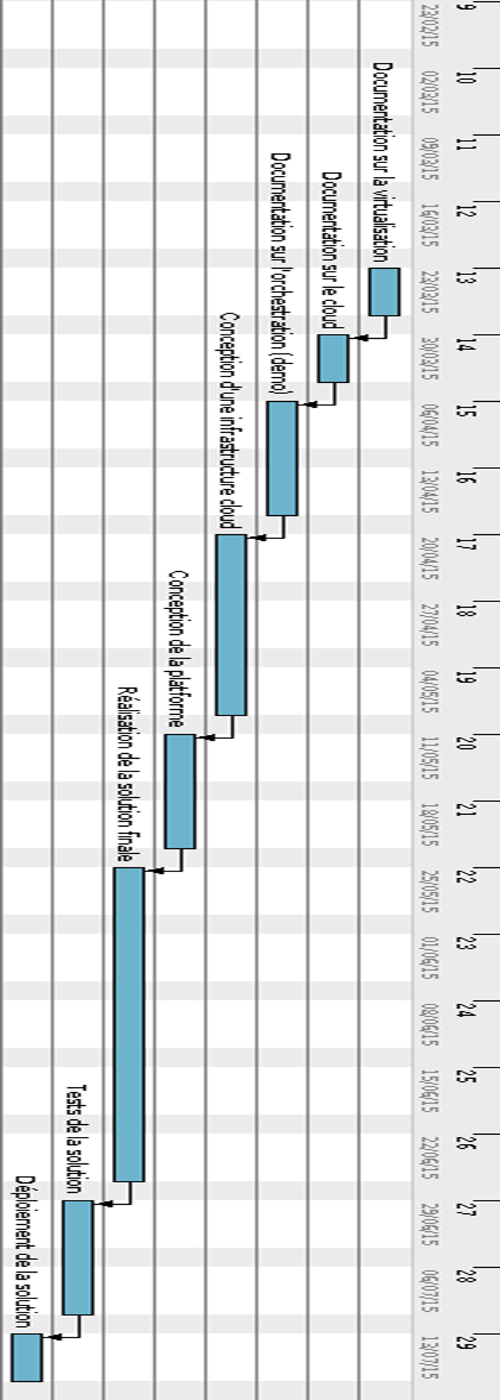
\includegraphics [scale=0.5]{chapitre1/assets/gantt.png}
\caption{Diagramme de Gantt}
\end{figure}


\end{onehalfspace}

\chapter{Le cloud computing}
\begin{onehalfspace}

\initial{L} e but de ce chapitre est d'exposer le travail fait au niveau de la documentation. Ce chapitre est très riche par des concepts incontournables à la suite de ce rapport. En effet, nous allons commencer par expliquer ce que signifie le cloud concrètement. Ensuite nous présenterons les types de cloud les plus classiques, à savoir IaaS, PaaS et SaaS. Enfin, les notions machines virtuelles et conteneurs seront présentées avec une comparaison détaillée des deux.


\newpage


\section{Le Cloud Computing}

\subsection{Définition}

Le \textbf{Cloud Computing} est l'exploitation de la puissance de calcul ou de stockage de serveurs informatiques distants par l'intermédiaire du réseau internet. Ces serveurs sont loués à la demande selon des critères technique (Bande passante, puissance, etc.). Le cloud computing se caractérise par sa grande souplesse. En effet, il est déstiné aux utilisateurs de tous les niveaux de compétences.

Le cloud est rendu possible grâce à la virtualisation, l'ubiquité des réseaux à grande vitesse, les capacités des navigateurs d'aujourd'hui et l'évolution des piles de développement Web. Avec ces choses en place, il devient moins nécessaire de posséder votre propre infrastructure, ou même de posséder votre propre logiciel. Vous pouvez obtenir ce que vous avez besoin à partir du Cloud, tant que vous en avez besoin.


\subsection{Caractéristiques}

En termes clairs, le Cloud donne la capacité pour les utilisateurs finaux d'utiliser des pièces de ressources. Ces ressources doivent être acquises rapidement et facilement. NIST définit plusieurs caractéristiques qu'il juge essentiel pour qu'un service soit considéré comme «Cloud». Ces caractéristiques comprennent:

\begin{itemize}

\item Service à la demande. La capacité pour un utilisateur final de s' inscrire et recevoir des services sans les longs délais qui ont caractérisé l'informatique traditionnelle;

\item Accessible au réseau large. La Capacité d'accéder au service via les plates-formes standard (bureau, ordinateur portable, mobiles, etc.);

\item La mise en commun des ressources. Les fournisseurs servent plusieurs clients ou «locataires» avec des services provisoires et scalables. Ces services peuvent être ajustés pour répondre aux besoins de chaque client, sans aucune modification apparente pour l'utilisateur;

\item Rapide élasticité. La capacité des ressources doit évoluer pour faire face aux pics de la demande;

\item Service mesuré. La facturation est mesuré et livré


\end{itemize}

Sans ces caractéristiques, l'informatique en nuage n'appore rien par rapport à l'informatique traditionnelle. Une solution Cloud doit démontrer ces caractéristiques et notre projet ne doit pas échapper à cette règle. Dans ce qui suit, nous détaillerons les types classiques du cloud.

\subsection{Les types de Cloud}

Le Cloud Computing est un large terme qui décrit une large collection de services. Dans ce rapport, nous allons expliquer les différents types de services de Cloud communément appelé Software as a Service (SaaS),  Platform as a Service (PaaS) et Infrastructure as a Service (IaaS) et décrirent plus en détails ceux qui touchent à notre sujet.

\begin{figure}[H]
\centering
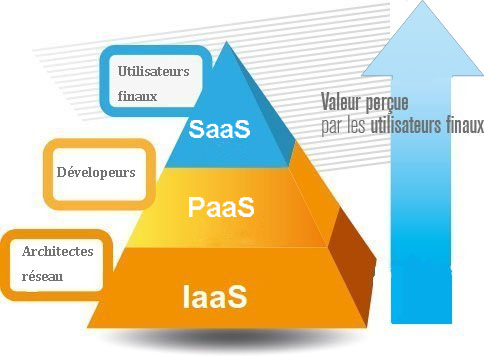
\includegraphics [scale=0.7]{chapitre2/assets/pyramide.jpg}
\caption{Pyramide des services Cloud}
\end{figure}

\subsubsection*{Software as a Service}

La meilleure façon de comprendre ces services est de commencer avec le SaaS, la couche la plus abstraite et celui qu'on utilise peut-être déjà aujourd'hui, même à un niveau personnel. Un exemple simple de SaaS est un service de messagerie en ligne, comme Gmail. Lorsque l'on utilise Gmail, vous n'êtes pas hébergez votre propre serveur de messagerie. C'est Google qui l'héberge, et on est tout simplement entrain d'y accéder via un navigateur comme un client.

SaaS est vraiment orienté vers les utilisateurs finaux de l'entreprise et ne nécéssite pas beaucoup de compétences pour l'utiliser. Le fournisseur décide sur le nombre de ressources à consacrer à l'utilisation de l'application. Le fournisseur décide sur les serveurs, les machines virtuelles, l'équipement de réseau, tout. Enfin, il suffit de pointer le navigateur à l'application.

\subsubsection*{Infrastructure as a Service}

IaaS est à l'autre bout du pyramide du Cloud. Lorsque l'on souhaite garder le contrôle de l'environnement logiciel, mais on veut pas maintenir aucun équipements; Lorsque l'on veut pas acheter des serveurs et de les mettre dans une pièce à température contrôlée ou rien de tout cela; On va chez un fournisseur IaaS et demander tout simplement une machine virtuelle.

L'on peut mettre n'importe quel logiciel que l'on souhaite au-dessus d'IaaS. Sur l'arrière, le fournisseur obtient vous de stockage ou d'autres ressources que l'on a besoin. Ceci est rendu plus facile avec les technologies de virtualisation, qui séparent les ressources physiques de la machine virtuelle qui éxécute le logiciel. IaaS est disponible sur Amazon EC2, GCE de Google et bien d'autres.

L'infrastructure en tant que service ou l'IaaS ne touche pas directement à notre sujet. Du coup, il ne sera mentionné que rarement par la suite.

\subsubsection*{Platform as a Service}

PaaS se situe quelque part entre IaaS et SaaS. Il est pas un produit fini, comme SaaS, encore moins une simple ressource virtuelle vierge, comme IaaS. PaaS est destiné pour les développeurs, il leur donne des outils et des interfaces de haut niveau pour y développer dessus. Par exemple, Windows Azure de Microsoft vous donne des outils pour développer des applications mobiles, des applications sociales, sites Web, jeux et plus encore. Vous construisez ces choses, mais vous utilisez les API et les outils pour les accrocher dans l'environnement Azure et de les exécuter là.


\begin{figure}[H]
\centering
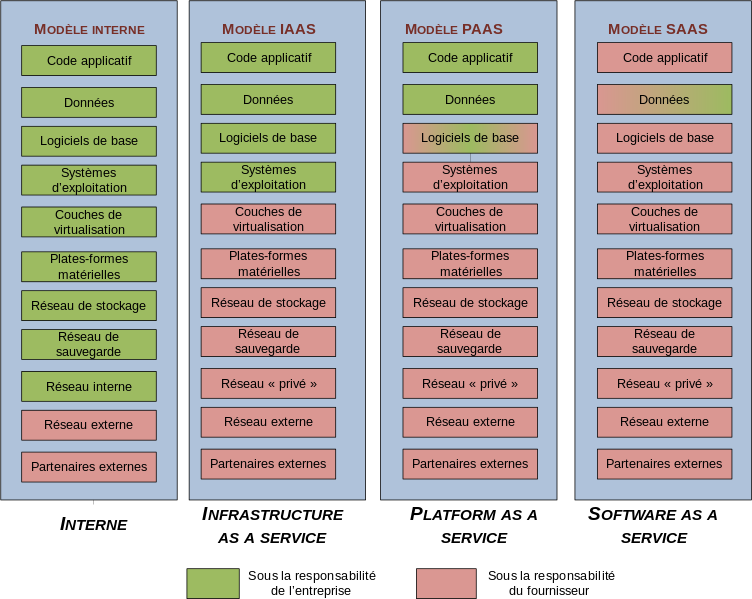
\includegraphics [scale=0.5]{chapitre2/assets/cloud-vs.png}
\caption{L'éxternalisation de l'informatique en Cloud}
\end{figure}


\section{Virtualisation ou containérisation}

\subsection{Virtualisation}

Avec des racines profondément ancrées dans l'informatique, la virtualisation sert à partitionner un seul serveur physique en plusieurs machines virtuelles, comme un espace de stockage ou un réseau, en plusieurs ressources virtuelles. Elle permet une consolidation de serveurs avec une grande souplesse d'utilisation. Dans le contexte de l'informatique en nuage, la virtualisation est importante pour la mise en service et le retrait rapide de serveurs. Ceci étant dit, la scalabilité est la principale caractéristique du Cloud moderne, faute de cela, on ne peut en parler. Ainsi la virtualisation a permis de créer des machines virtuelle, les faire monter en charge à la demande, faire de la migration à chaud, etc. La virtualisation est une technologie permettant d'arriver à une utilisation rentable des serveurs tout en prenant en charge la séparation entre de multiples locataires d'un matériel physique.

Il existe plusieurs solutions de virtualisation, l'on peut citer à titre informatif:

\begin{itemize}
\item VMware, Cette solution, séduisante, pose certains problèmes. En effet, il propose des outils propriétaires et incompatible avec le noyau Linux;
\item Xen est un hyperviseur libre de machines virtuelles, il est considéré comme un outil de virtualisation des plus performants;
\item KVM, Kernel-based Virtual Machine est devenue rapidement la solution de virtualisation de référence pour Linux. Elle est basée sur les architectures Intel ou les architectures AMD;
\item QEMU, est un émulateur machine générique. C'est une solution de virtualisation à utiliser si le processeur de système hôte ne possède pas d'extension matérielle spécifique à la virtualisation.

\end{itemize}

\subsection{Containérisation}

Noyau Linux permet de lancer plusieurs instances isolées de l'espace utilisateur. Un conteneur est un environnement isolé où un ou plusieurs processus peuvent être exécutés. Les conteneurs se concentrent sur l'isolation des processus au lieu d'émuler une machine physique complet.

Historiquement, chroot dans le noyau Linux a fourni un certain niveau d'isolation en fournissant un environnement pour créer et héberger une copie virtualisée d'un logiciel, et ceci depuis le début des années 80. Mais le terme «conteneurs» n'est pas venu jusque vers la fin de l'année 2006. Il a été renommé «Control Groups» (cgroups) pour éviter toute confusion causée par de multiples significations du terme «conteneurs» dans le noyau Linux. «Control Groups est une fonctionnalité du noyau linux qui est disponible depuis la version v2.6.24, elle limite et isole l'utilisation des ressources d'un ensemble de processus. Par la suite, l'isolation de l'espace de noms a été ajouté.

Cela a conduit à l'évolution de Linux Containers (LXC), un environnement de virtualisation au niveau du système d'exploitation qui est construit sur les fonctionnalités du noyau Linux mentionnés plus haut, comme chroot, cgroupes, l'isolation de l'espace de noms, etc.

\paragraph{Cgroups}

\begin{itemize}
\item Isolation de l'usage des ressources (CPU, mémoire, E/S, etc.);
\item Limitation des ressources: un groupe peut être configuré pour ne pas dépasser une certaine limite de la mémoire;
\item Priorité: certains groupes peuvent obtenir une plus grande part de CPU ou de débit E/S disque;
\item Mesure de l'usage des ressources;
\item Contrôle: le gel des groupes ou des points de reprise et le redémarrage.
\end{itemize}

\paragraph{Namespaces}
\begin{itemize}
\item Partionnement des structures de kernel pour créer des environnements virtuels
\item Des espaces de noms différents

\begin{itemize}
\item pid (processus)
\item net (interfaces réseaux, routage, ...)
\item ipc (communication inter-processus)
\item mnt (points de montage, système de fichiers)
\item uts (Nom de hôte)
\item user (UIDs)
\end{itemize}

\end{itemize}


\paragraph{}
Contrairement à la virtualisation, la liste des solutions de containérisations n'est pas aussi longue. La plupart d'eux se basent sur ou convergent vers cgroups et namespaces. L'on cite:

\begin{itemize}
\item LXC, Linux containers, combine cgroups et namespace pour fournir un environnement isolé pour les applications;
\item OpenVZ permet de créer multiples conteneurs pour Linux. Dorénavant, tous les efforts des développeurs d'OpenVZ vont aller dans le sens de fusionner les fonctionnalités d'OpenVZ avec LXC;
\item lmctfy, Let Me Contain That For You, est une solution open source de containérisation de Google qui est basé sur cgroups. Le futur de lmctfy est flou vu que Google avait commencé à migrer les concepts de lmctfy vers Docker;
\item Docker, ce n'est pas une autre solution, mais il est basé sur LXC et fournit une couche de haut niveau accessible pour l'utilsateur;

\end{itemize}

\subsection{Etude comparative}

Le choix de la solution a été proposé fortement par la société. On a opté pour une solution de containérisation (Docker) dans la mesure où un benchmark prouve son efficacité et sa légèreté.





\section{Docker}
\subsection{Présentation de Docker}
Docker est un logiciel open source qui automatise le déploiement d'applications dans des conteneurs logiciels. C'est un outil qui peut empaqueter une application et ses dépendances dans un conteneur virtuel, qui pourra être exécuté sur n'importe quel serveur Linux ou Windows (Boot2Docker). En fait, Docker a pour objectif de \textbf{faciliter le déploiement d’applications}, d’avoir plusieurs versions d’une même application sur un son serveur (phase de développement, tests), mais aussi d’\textbf{automatiser le packaging d’applications}. Avec Docker, on s’oriente vers de l’intégration et du déploiement en continu grâce au système de container. De plus, Docker permet de garder son système de base propre, tout en installant de nouvelles fonctionnalités au sein de containers, on part d’une base qui est le système d’exploitation et on ajoute différentes briques conteneurisées. Docker a été distribué en tant que projet open source à partir de mars 2013.
\begin{figure}[H]
\centering

\includegraphics [scale=0.5]{chapitre2/assets/docker.png}
\caption{Logo de Docker}
\end{figure}

\subsection{Utilisation de Docker}
Docker propose de nombreux templates qui permettent de déployer des applications en container, très rapidement. La communauté est très active, ce qui permet aux utilisateurs de disposer de nombreux containers applicatifs préfaits.
Docker est basé sur LXC (Linux Containers) qui est une référence sous Linux quant à l’utilisation des containers. Par ailleurs, Docker intègre les éléments suivants :
\begin{itemize}
\item \textbf{Control Groups} : Fonctionnalité du noyau Linux pour limiter, compter et isoler les ressources (CPU, RAM, etc.) utilisées par un groupe de processus.
\item \textbf{AppArmor et SElinux} : Gestion avancée des permissions aussi bien au niveau des applications qu’au niveau du système de fichiers.
\item \textbf{Kernel namespace} : Fonctionnalité du noyau Linux qui permet l’isolation, afin de s’assurer qu’un container ne puisse pas en affecter un autre.
\item \textbf{chroot} : Fonctionnalité qui permet de changer la racine d’un processus, afin de l’isoler sur un système par mesure de sécurité.
\end{itemize}

Docker propose des services pour effectuer facilement différentes actions : créer, éditer, publier et exécuter des containers. On parlera souvent des notions de containers, images et dockerfiles.

\begin{itemize}
\item \textbf{DockerFile} : Fichier source qui contient les instructions, éléments à installer, c’est un fichier de configuration.
\item \textbf{Image} : Compilation d’un fichier DockerFile pour former une image portable, prête à être déployée.
\item \textbf{Container} : Exécution d’une image, mise en container d’une image.
\end{itemize}


Le schéma suivant décrit le fonctionnement de l'outil \emph{Docker}: 
\begin{figure}[H]
\centering
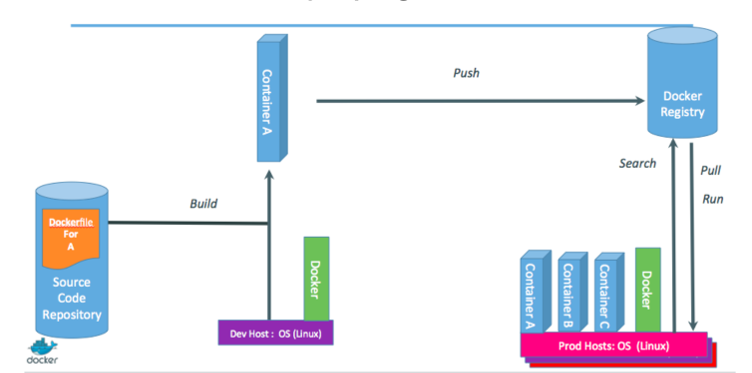
\includegraphics [scale=0.6]{chapitre2/assets/utilisation.png}
\caption{Fonctionnement de Docker}
\end{figure}

\end{onehalfspace}
\chapter{Orchestration des applications distribuées}
\begin{onehalfspace}

\initial{D}ocker est un outil qui a révolutionné le monde informatique par l'introduction de la notion de conteneur, donc il est normal de chercher à l'utiliser en production. De nos jours, les développeurs utilisent de plus en plus Docker pour déployer des applications qui s’exécutent sur plusieurs conteneurs et plusieurs hôtes. Orchestrer ces applications distribuées nécessite une approche \textbf{multi-conteneur} et \textbf{multi-hôte} native avec une interface utilisateur et de l'outillage commun qui fonctionnent sur toutes les infrastructures. Plusieurs outils ont été présentés par de grandes entreprises et qui sont toujours en cours de développement. Nous exposerons dans ce chapitre les projets promoteurs dans l'orchestration des applications distribuées.

\newpage

\section{Le Clustering}

\index{Cluster}

Nous avons présenté dans le chapitre 2 le Cloud Computing ainsi que ses services classiques. Dans cette section, nous allons parler du cluster comme un service et le situer dans le pyramide des services du Cloud (Figure ~\ref{fig:pyramide-cluster}).

\begin{figure}[H]
\centering
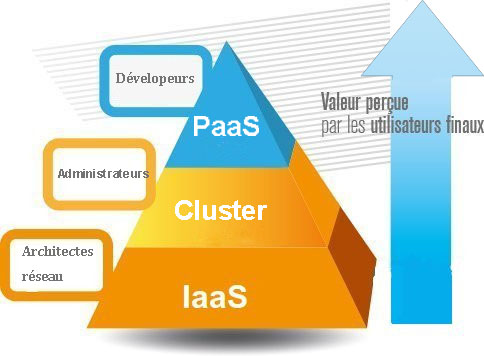
\includegraphics [scale=0.7]{chapitre3/assets/pyramide}
\caption{Le Cluster dans le Cloud}
\label{fig:pyramide-cluster}
\end{figure}

\begin{itemize}
	\item \index{PaaS} \textbf{Plate-forme}: Un développeur crée une application dans un ensemble particulier de langages de programmation à l'aide des \acrshort{api}s spécifiques et pousse ce code vers la plate-forme. La plate-forme l'exécute et lance une seule copie du service ou éventuellement plusieurs copies dépendamment du trafic. Finalement ce service monte en charge automatiquement. 
	\item \index{IaaS} \textbf{\acrshort{iaas}}: A l'autre bout du pyramide se trouve l'\acrshort{iaas} composé seulement de machines virtuelles qui résident essentiellement dans l'internet. Quand un utilisateur consulte un fournisseur \acrshort{iaas} et demande  un ordinateur avec des spécifications données (quantité de mémoire et de disque, nombre de \acrshort{cpu}, une version spécifique Linux, etc). En quelques minutes, L'utilisateur pourra  exécuter n'importe quel logiciel sur le serveur mais il est entièrement responsable de la gestion de la machine.
	\item \textbf{Cluster}: C'est lorsqu'il y a un besoin de gérer un ensemble de machines, un cluster de machines comme une seule entité, pas seulement un ordinateur individuel (\acrshort{iaas}) et non plus toute une plate-forme magique.

\end{itemize}


\def\arraystretch{1.6}%  1 is the default, change whatever you need

{\rowcolors{1}{tabOdd}{tabEven}
\begin{center}
\begin{table}[H]

	\begin{tabu}{| X[c] | X[c] | X[c] | X[c] |} 


	\hline
	\rowcolor{tabHead}
	\textbf{} & \textbf{IaaS (VMs)} & \textbf{Cluster} & \textbf{Plate-forme}\\ [0.95ex] 
	\hline\hline
	A quoi sert ? 	& Créer et déployer les images des machines virtuels & Créer et déployer des conteneurs & créer et déployer des applications (services) \\ 
	Automatise					& - & Ordonnancement & Tout \\ 
	gére					& Un seul atome & Des serveurs & Des applications \\ 
	fléxibilité					& ++ 	& + 	& - \\ 
	Agilité						& - 	& + 	& ++ \\ 
	\hline
	\end{tabu}
	\caption{Le Cluster dans le Cloud}
	\label{tab:table_label}

\end{table}
\end{center}
}


En général, un cluster comporte plusieurs éléments qu'on définit ci-dessous :

\begin{itemize}
	\item \textbf{Master} : C'est la machine qui est responsable du Cluster. Il veille sur son bon fonctionnement grâce au système de découverte des services et l'ordonnanceur
	\item \textbf{Ordonnanceur} : Dans un ordinateur ordinaire, pour démarrer un processus, on a besoin d'un gestionnaire des processus pour les faire fonctionner et les garder en cours d'exécution. L'ordonnanceur le fera sur l'ensemble des machines (Cluster)
	\item \textbf{Nœud} : Une machine qui appartient au Cluster, elle peut être réelle ou virtuelle.
	\item \textbf{Gestionnaire des conteneurs} : C'est la partie de logiciel qui est distribuée dans chaque machine du cluster. Il supervise les conteneurs ordonnancés, les redémarrent en cas de nécessité.
	\item \textbf{Conteneurs ordonnancés} : Un service fonctionne à l'intérieur d'un conteneur ordonnancé. En effet, ce conteneur se trouve dans une telle machine  parce que le développeur a déclaré à l'ordonnanceur du Cluster (maître) les besoins du service en terme de ressources (nombre de CPU, RAM, etc...). L'ordonnanceur fournit pour le service un endroit où il peut vivre en paix.
\end{itemize}


\begin{figure}[H]
\centering
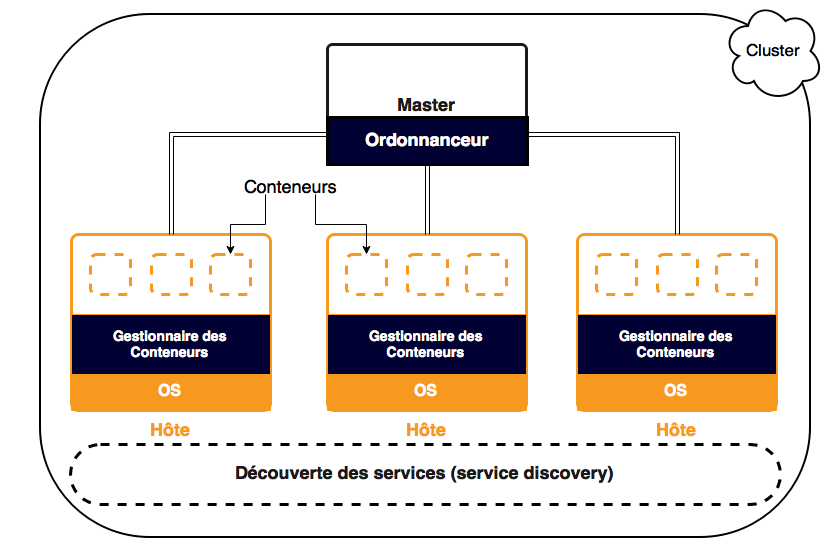
\includegraphics [scale=0.55]{chapitre3/assets/cluster}
\caption{Un cluster en général}
\label{fig:}
\end{figure}

Nous avons vu la notion de cluster et les processus d'automatisation et coordination. De ce fait, la gestion des services informatiques distribués se trouve incontournable au fonctionnement du cluster, elle est appelé \textbf{l'orchestration}. Dans la section suivante, nous allons détailler les différents solutions d'orchestration qui existent dans le monde de la containérisation.

\section{Orchestration Docker}
Les capacités d'orchestration de Docker sont construites sur les fondations existante de Docker. Ces capacités sont assurées par trois nouveaux services de la plate-forme qui sont conçus pour couvrir tous les aspects du cycle de vie dynamique des applications distribuées. Selon l'entreprise Docker, toutes ces caractéristiques sont conçues avec la philosophie de conception "\emph{Batteries Included, but Removable}" qui indique qu'ils peuvent fonctionner avec des services tierces. Ceci offre le choix aux clients de choisir entre les différents outils d'orchestration de Docker et les alternatives communautaires.


%\begin{figure}[H]
%\centering
%
\includegraphics [scale=0.4]{chapitre3/assets/orchestrationdocker.png}
%\caption{Orchestration Docker}
%\end{figure}
\subsection*{Docker Machine}
 Ce service facilite le provisionnement d'un hôte avec Docker installé dans une variété d'environnements. Les développeurs peuvent rapidement lancer les machines hôtes exécutant Docker ; sur un ordinateur portable, un Datacenter de VMs, ou une instance Cloud. Cela évite la tâche de se connecter à un hôte pour installer et configurer le démon Docker et le client. Bien que toujours en version alpha, Docker machine prend en charge le provisionning de Docker localement avec VirtualBox et à distance sur les instances Digital Ocean. Le support pour AWS, Azure, VMware, OpenStack et d'autres infrastructures devrait arriver rapidement.
 \begin{figure}[H]
\centering
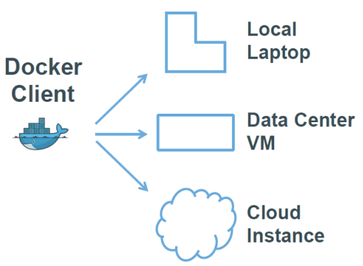
\includegraphics [scale=0.6]{chapitre3/assets/dockermachine.png}
\caption{Docker Machine}
\end{figure}
\subsection*{Docker Swarm}
 Docker Swarm est un service de Clustering natif de Docker qui fonctionne avec l'engine Docker standard, et qui crée un pool de ressources sur lesquels les applications distribuées s'exécutent. Cela permet aux développeurs et équipes opérationnelles de considérer un cluster de machines Docker comme un pool de ressources unique. Les administrateurs peuvent planifier des conteneurs qui seront lancés dans l'un des hôtes qui répond aux exigences. Docker Swarm fournit des contraintes standard et personnalisées pour répondre aux besoins et à la planification basée sur des règles, cela permet de déclarer des exigences et contraintes spécifiques à chaque conteneur. Docker Swarm est conçu pour évoluer avec le cycle de vie de l'application. Il peut prendre en charge un hôte dans l'environnement de développement et d'autres s'exécutant dans l'environnement de production.
\begin{figure}[H]
\centering
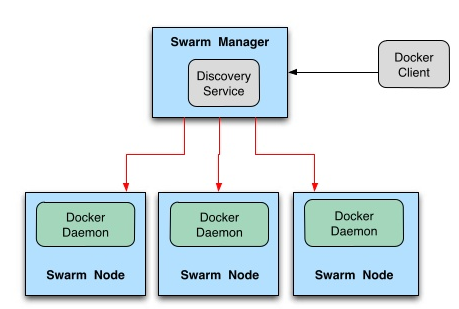
\includegraphics [scale=0.6]{chapitre3/assets/dockerswarm.png}
\caption{Architecture de Docker Swarm}
\end{figure}
\subsection*{Docker Compose}
  Docker Composer permet aux développeurs d'assembler des applications de conteneurs autonomes, interopérables et indépendants de l'infrastructure sous-jacente. Avec cette approche déclarative, il est facile de définir des stacks qui sont portables. Une stack d'applications distribuées est déclarée à travers un simple fichier de configuration \acrshort{yaml} qui contient la définition de chaque conteneur.
\begin{figure}[H]
\centering
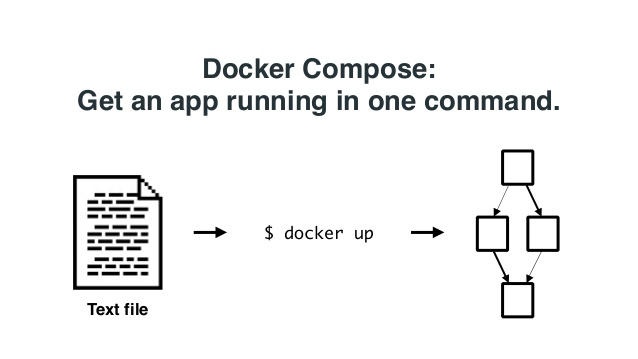
\includegraphics [scale=0.5]{chapitre3/assets/dockercompose.jpg}
\caption{Docker Compose}
\end{figure}
\section{Orchestration Google}

\index{Kubernetes}

L'entreprise Google est aussi intéressée par l'orchestration des conteneurs docker, elle a d'ailleurs lancée un projet nommée \textbf{Kubernetes}.Ce projet est récent mais promoteur et pourrait révolutionner le domaine du Cloud s'il est suffisamment mature pour la production. Kubernetes a pour objectif de fournir un outil de supervision unique capable de déplacer des conteneurs Docker d'un Cloud à un autre. Autrement dit, de proposer une forme d’interopérabilité dans le nuage, via un framework de gestion de conteneurs solide, ouvert et adapté à toute application sur tous types d’environnements, qu’il s’agisse de Cloud privé, public ou hybride. Ce projet a le soutien et l'attention des géants du Cloud notamment Microsoft, IBM, RedHat qui tiennent à s'assurer que cet outil sera compatible avec leurs Clouds et tentent de l'associer au projet \textbf{Openstack} qui est l'orchestrateur du cloud hybride open source.
\subsection{Architecture de Kubernetes}
Kubernetes est un outil open-source pour l'orchestration des conteneurs Docker. Il gère l'ordonnancement des nœuds dans un Cluster et gère les ressources pour mieux correspondre à l'intention de l'utilisateur. En utilisant les concepts de "\emph{labels}" et "\emph{pods}", il permet un regroupement optimal de conteneurs pour une meilleure gestion et une découverte facile.
\begin{figure}[H]
\centering
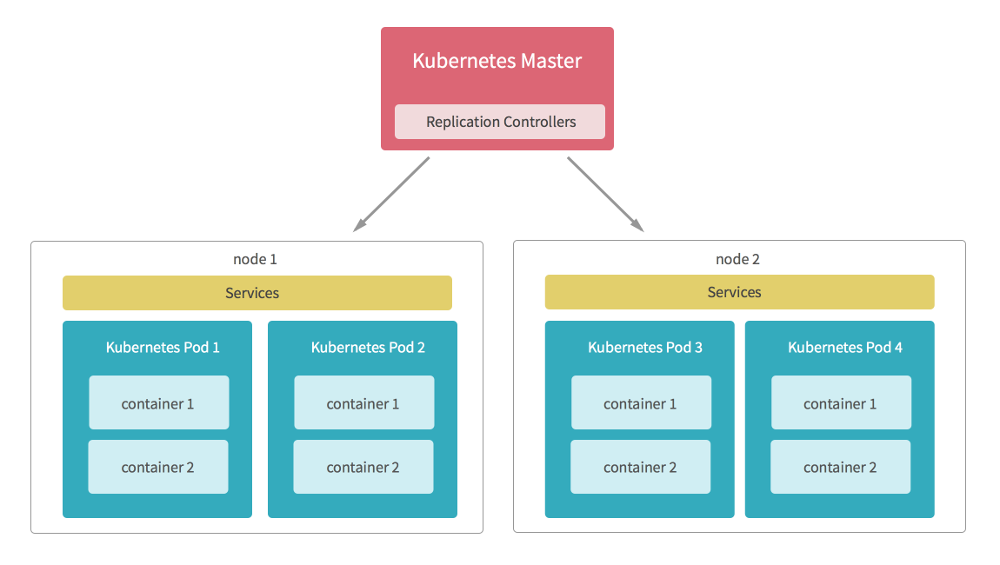
\includegraphics [scale=0.4]{chapitre3/assets/archkuber.png}
\caption{Architecture de Kubernetes}
\end{figure}

\begin{itemize}
\item \textbf{Kubernetes Master} : il contrôle l'ensemble du Cluster et exécute l'API. Fondamentalement, il est responsable du Cluster.

\item \textbf{Nodes} : un nœud est un serveur physique (ou une machine virtuelle) à l'intérieur du cluster. Il communique avec les maîtres et contient des conteneurs, on peut ajouter ou supprimer des nœuds à volonté.

\item \textbf{Pods} : un "\emph{Pod}" est le bloque basique de construction dans \emph{Kubernetes}.Dans un pod, il est possible de lancer plusieurs conteneurs. L'allocation des CPU, mémoire et des autres ressources est gérée dans un pod. Chaque pod possède sa propre adresse ip et son nom d'hôte pour éviter d'éventuels conflits de ports.

\item \textbf{Replication Controller} : Il est vrai que le Pod est un composant puissant au sein de \emph{Kubernetes} mais il ne permet pas la gestion des échecs. Les échecs sont des événements inévitables bien qu'il faudrait que le service soit toujours disponible. C'est de ce fait qu'intervient \emph{Replication Controller}. Ce dernier s'assure qu'un nombre donné de pods sont exécutés au sein du Cluster, il peut enlever et ajouter des pod du Cluster donc il faudra définir un pod template pour assurer sa fonction.

\item \textbf{Services} : les Pods sont ajoutés ou supprimés donc il faudrait permettre un \textbf{load-balancing} du trafic dans ses pods. "\emph{Service}" agit comme un \emph{load-balancer} dynamique pour un ensemble de pods, il est très efficace et utilise différentes techniques ( IP Tables, ...) pour éviter la surcharge.

\end{itemize}
%\begin{figure}[H]
%\centering
%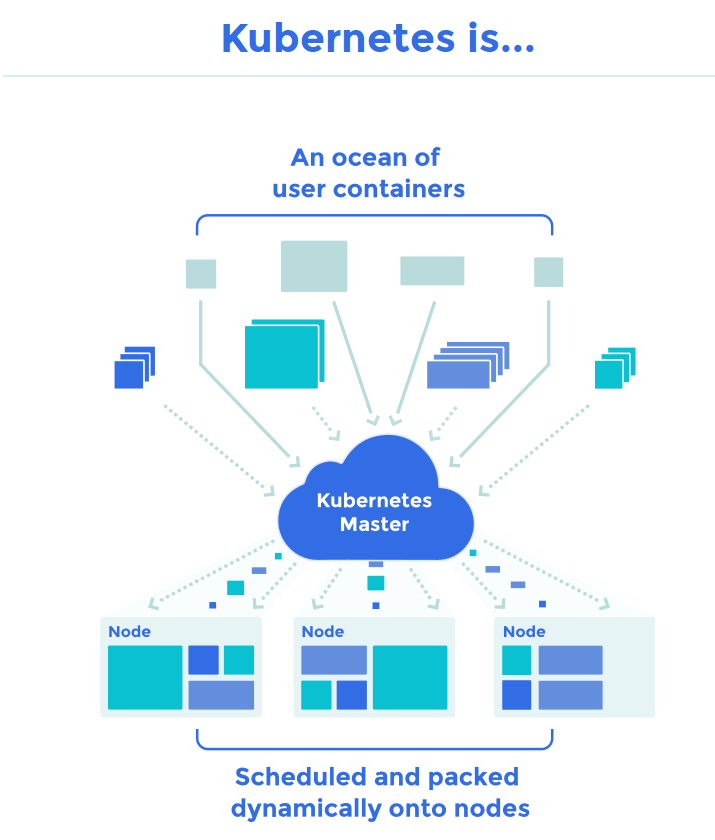
\includegraphics [scale=0.5]{chapitre3/assets/kuber.png}
%\caption{Résumé de Kubernetes}
%\end{figure}

\section{Orchestration Apache}

\index{Mesos}

L'entreprise Apache a toujours été intéressée par le domaine du Cloud, le lancement de son projet \textbf{Mesos} visait principalement à améliorer l'orchestration des \emph{"datacenters"} ceci bien avant l’émergence des conteneurs et docker. Le projet Mesos est très promoteur pour le futur avec les conteneurs bien qu'il soit déjà mature avec les machines virtuelles. Plusieurs grandes entreprise utilisent Mesos notamment \emph{Twitter}, \emph{Paypal} et \emph{Airbnb}.
Mesos agit comme un "Cluster Manager" et offre de nombreuses fonctionnalités telles que :
\begin{itemize}
\item Une scalabilité à plus de 10000 nœuds.
\item Isolement des ressources pour les tâches via les conteneurs linux (LXC).
\item Gestion efficace du CPU et de la mémoire interne.
\item Haute disponibilité du master via Apache Zookeeper.
\item Une interface Web pour le monitoring des Clusters.
\end{itemize}
\subsection{Architecture de Mesos}
\emph{Mesos} possède une architecture composée principalement de maîtres, esclaves et frameworks. Nous définirons dans cette partie les composants pertinents de l'architecture suivante.
\begin{figure}[H]
\centering
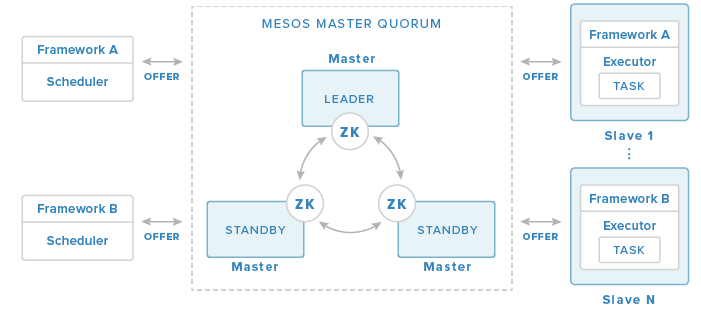
\includegraphics [scale=0.65]{chapitre3/assets/mesosarch.png}
\caption{Architecture de Mesos}
\end{figure}
\begin{itemize}
\item \textbf{Master daemon} : il tourne dans noeud "master" et gère les esclaves.
\item \textbf{Slave daemon} : il tourne aussi dans un noeud "master" et exécute les tâches des frameworks.
\item \textbf{Framework} : connu aussi par l'application Mesos, il est composé d'un ordonnaceur qui gère les offres d'allocation de ressources, et d'un ou plusieurs exécuteurs qui lancent les tâches sur les esclaves.
\item \textbf{Offer} : c'est une liste des ressources disponibles de la mémoire et du CPU propre à un nœud esclave. Tous les nœuds esclaves envoient des offres pour le maître  et ce dernier les transmet aux frameworks disponibles.
\item  \textbf{Task} : c'est un tâche qui est ordonnancée par un framework et qui est exécutée dans un nœud esclave. Cette tâche peut être de n'importe quel type (commande, script bash ,requête SQL, Hadoop Job, ...)
\item \textbf{Apache ZooKeeper }: C'est un logiciel qui coordonne les nœuds maîtres.
\end{itemize}
\subsection{Frameworks Mesos}
Le framework ou l'application Mesos tient une importante place au sein de l'architecture. Dans cette partie , on présentera deux frameworks importants qui sont \textbf{Marathon} et \textbf{Chronos}.
\begin{figure}[H]
\centering
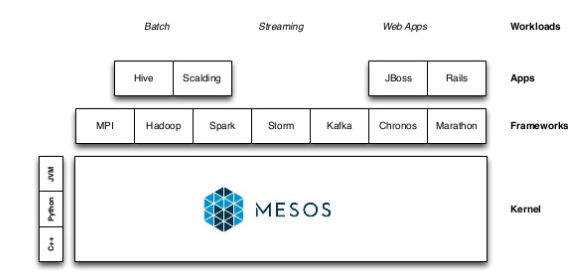
\includegraphics [scale=0.65]{chapitre3/assets/framework.png}
\caption{Composants de l'architecture Mesos}
\end{figure}
\subsubsection*{Marathon}
\emph{Marathon} est un framework Mesos développé pour exécuter les applications "\emph{long-running}". Il sert de remplacement pour le système \emph{init}. Il possède de nombreuses fonctionnalités qui simplifient les applications en cours d'exécution dans un environnement en Cluster telles que la haute disponibilité, les contraintes de nœuds, les contrôles de santé de l'application, une API pour scriptabilité et la découverte de service ainsi qu'un outil facile à utiliser l'interface utilisateur Web UI. Il ajoute ses capacités de mise à l'échelle et d'auto-guérison à l'ensemble des fonctionnalités de Mesos. 
\subsubsection*{Chronos}
\emph{Chronos} est une application Mesos qui a été initialement développé par Airbnb comme remplacement pour le système \emph{cron}.Il est un ordonnanceur pleinement fonctionnel , distribué et tolérant aux pannes pour \emph{Mesos}, ce qui facilite l'orchestration des "\emph{jobs}" qui sont des collections de tâches . Il comprend une API qui permet d'exécuter les scripts de la planification de tâches et une interface web pour la facilité d'utilisation.
\emph{Chronos} est complémentaire à \emph{Marathon} car il fournit une autre façon d'exécuter des applications selon un calendrier ou d'autres conditions telles que la réalisationn d'un autre emploi. Il est également capable de la planification de tâches sur plusieurs nœuds esclaves \emph{Mesos}, et fournit des statistiques sur les échecs et les réussites d'emploi.
\section{Coreos}
\index{CoreOS}
\textbf{Coreos} est un système d'exploitation open-source basé sur le noyau \emph{Linux} et construit pour fournir des infrastructures aux déploiements en Cluster. En effet, il est un système minimaliste, sur lequel est greffé des conteneurs applicatifs indépendants et sécurisés. Coreos est conçu pour être léger et performant afin de gérer les datacenters. Coreos consomme 40\% moins de mémoire au démarrage en moyenne par rapport à un serveur \emph{Linux}. Coreos est disponible sur plusieurs plates-formes comme Amazon Compute Cloud, Google Compute Engine et plusieurs autres.
%\begin{figure}[H]
%\centering
%
\includegraphics [scale=0.4]{chapitre3/assets/logocoreos.png}
%\caption{Logo de Coreos}
%\end{figure}
\subsection{Composants de Coreos}
\subsubsection*{Le service Systemd}
\index{Systemd}
\emph{systemd} est une suite de gestion de système, de bibliothèques et utilitaires conçus comme un système central de management et configuration pour le système d'exploitation Linux. Il est contrôlé dans le système d'exploitation Coreos par le service \emph{Fleet}.
\subsubsection*{Le service Etcd}
\index{Etcd}
Le service \emph{etcd} est une base de données distribuée de clé-valeur qui fournit une configuration partagée et un service de découverte pour les Clusters \emph{Coreos}.Il fonctionne sur chaque machine dans un Cluster et gère l'élection du maître lors des partitionnements réseaux ou la perte du maître.
\begin{figure}[H]
\centering
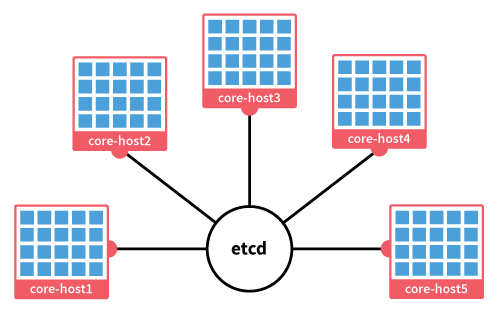
\includegraphics [scale=0.4]{chapitre3/assets/etcd-cluster.png}
\caption{Service etcd.}
\end{figure}
\subsubsection*{Le service Fleet}
\index{Fleet}
\emph{Fleet} permet de traiter le Cluster \emph{Coreos} comme s'il partageait un unique système d'initialisation. Il encourage les utilisateurs à écrire des applications sous forme de petites unités éphémères qui peuvent facilement migrer autour d'un Cluster. En utilisant \emph{Fleet}, les développeurs peuvent se concentrer sur la gestion des conteneurs sans soucier des machines qui tournent les conteneurs. Le service \emph{Fleet} a plusieurs avantages: 
\begin{itemize}
\item Déployer conteneurs docker sur des hôtes arbitraires dans un cluster.
\item Distribuer des services à travers un Cluster à l'aide de niveau machine anti-affinité.
\item Découvrir les machines fonctionnant dans le Cluster.
\item SSH automatiquement dans la machine exécutant un emploi.
\end{itemize}
\begin{figure}[H]
\centering
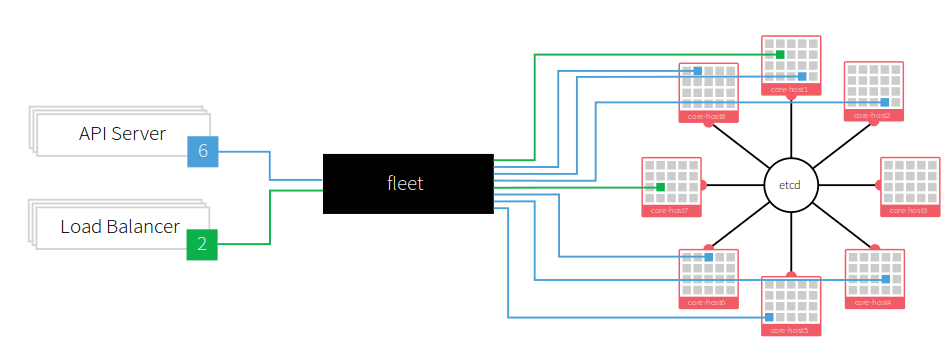
\includegraphics [scale=0.5]{chapitre3/assets/fleet.png}
\caption{Service management Fleet.}
\end{figure}
\end{onehalfspace}


\section{Récapitulation}


\def\arraystretch{1.6}%  1 is the default, change whatever you need

{\rowcolors{1}{tabOdd}{tabEven}
\begin{center}
\begin{table}[H]

	\begin{tabu}{| X[c] | X[c] | X[c] |} 


	\hline
	\rowcolor{tabHead}
	\textbf{CoreOS} & \textbf{Kubernetes} & \textbf{Mesos}\\ [0.95ex] 
	\hline\hline
	Etcd élit le leader du cluster 	& Un master par cluster & Haute disponibilité des masters \\ 
	Orchestration bas niveau & Orchestration haut niveau & Orchestration bas niveau \\ 
	Stable					& Version de pré-production & Stable \\ 
	Rapidité d’installation du cluster & Moins rapide & Moins rapide \\ 
	Bien documenté & Documentation pauvre & Bien documenté \\ 
	Inconscience vis-à-vis les ressources du cluster & Inconscience vis-à-vis les ressources du cluster & Ordonnancement conscient des ressources du cluster \\ 
	Axé sur les conteneurs & Il rassemble des années d’expériences de Google avec l'orchestration des conteneurs	& moins axé sur les conteneurs \\ 
	Destiné pour Docker & Destiné pour Docker	& Utilisé depuis des années pour l'orchestration de Hadoop, il vient de subir un ré-usinage de code pour supporter Docker \\ 
	Limité & Complet (encore plus dans le futur) & Management générique du cluster, extensibilité par les différents ordonnanceurs \\ 
	Pas de proxy et d'équilibreur de charge & Dispose de son propre proxy & Des proxy matures e,enfichables \\ 
	\hline
	\end{tabu}
	\caption{Matrice de décision pour le choix de la solution d'orchestration}
	\label{tab:table_label}

\end{table}
\end{center}
}


Mesos, Kubernetes et CoreOS essaient tous de résoudre des problèmes très similaires, chacun agit dans un niveau d'abstraction. L'on peut imaginer faire des combinaisons les trois solutions d'orchestration en cas de nécessité:

\begin{itemize}
	\item \textbf{CoreOS + Kubernetes}: CoreOS est parfait pour créer rapidement un Cluster. Il va ordonnancer les composants de base de Kubernetes dans le Cluster. L'ordonnancement des conteneurs va être délégué à Kubernetes.
	\item \textbf{Mesos + Kubernetes}: Mesos n'inclut pas nativement un ordonnanceur. L'extensibilité de Mesos fait qu'il est possible de laisser Kubernetes agir comme l'ordonnanceur de Mesos.
	\item \textbf{CoreOS + Mesos + Kubernetes}: L'idée est de jouir de tous les points forts des solutions. En contrepartie, on perd en simplicité, il est préférable de l'adopter qu'en cas de nécessité.
\end{itemize}

Faute de maturité, nous allons adopter CoreOS pour sa stabilité, sa simplicité et sa documentation disponible en dépit qu'il est bas niveau.
\chapter{Conception}
\begin{onehalfspace}

\newpage

\section{Base de donnée}



Odoo, comme toute autre application, a besoin d'une base de donnée \emph{PostgreSQL} pour persister des informations. Malheureusement, la communauté de Docker n'est pas si satisfaite vis-à-vis l'idée de containériser les bases de données. Nous allons prouver à travers deux scénarios qu'il serait une imprudence de tourner les bases de données dans des conteneurs.

Le fait de la rapidité et la légèreté de Docker et des conteneurs en général a poussé CoreOS d'adopter une certaine philosophie à l'égard de la gestion et l'ordonnancement des conteneurs. En effet, lorsqu'un conteneur s'est arrêté pour une raison quelconque, il va être automatiquement écrasé et remplacé par un nouveau qui va tourner le même service. Une philosophie, certes, moins prudente et parait naïve, mais sa simplicité épargne beaucoup de problèmes à tout le monde.

Par conséquent, on ne peut en aucun cas mettre les données dans le système de fichiers d'un conteneur sous peine de les perdre. La figure \ref{fig:database1} montre qu'après avoir tuer un conteneur, ses données sont perdues.

\begin{figure}[H]
\centering
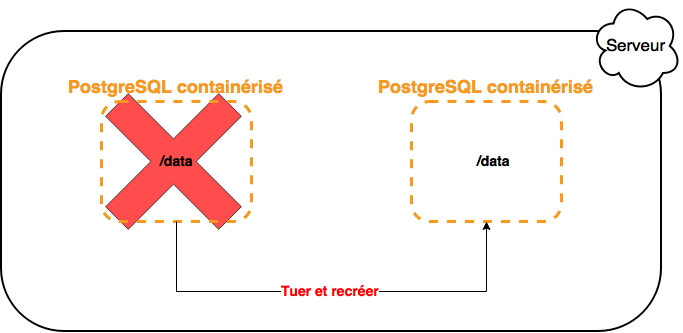
\includegraphics [scale=0.5]{chapitre4/assets/database1}
\caption{Données perdues - scénario 1}
\label{fig:database1}
\end{figure}

Pour y remédier, l'on peut penser à monter le volume des données dans le serveur hôte, ainsi les données sont plus ou moins persistées. Outre le fait que les données seront certainement perdues quand le serveur tombe en panne, le conteneur n'aura plus accès aux données quand il sera réordonnancé. En effet, le caractère imprévisible de l'ordonnanceur \emph{Fleet} fait qu'il n'y a pas de garantie qu'un conteneur réside dans le même serveur. La figure \ref{fig:database2} montre ce scénario.

\begin{figure}[H]
\centering
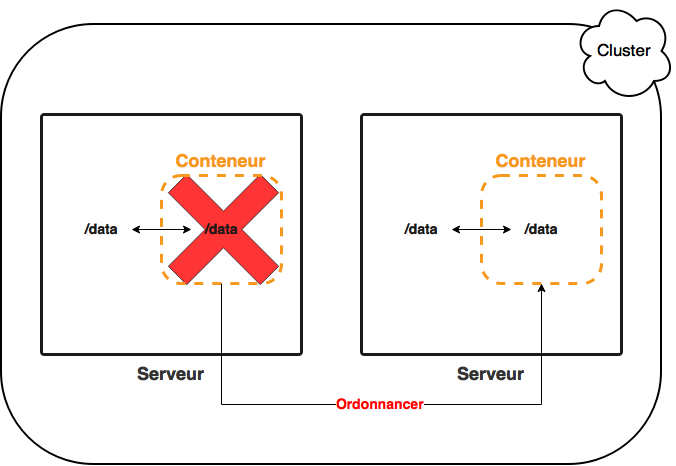
\includegraphics [scale=0.5]{chapitre4/assets/database2}
\caption{Données perdues - scénario 2}
\label{fig:database2}
\end{figure}


Dans un environnement de production, il est encore tôt pour mettre les bases de donnée et les applications à états (stateful) en général dans des conteneurs. De ce fait, il serait judicieux de les faire sortir de l'architecture à base de conteneurs. En effet, deux solutions se portent à nous, les bases de données vont être mis en place suivant l'informatique classique ou elles vont être consommées comme un service à partir d'une partie tierce cloud (Délégation de l'informatique). La dernière solution est couteuse mais il est plus fiable.



\section{Scalabilité et disponibilité}


Parmi les contraintes qui ont poussé Sayoo à migrer vers le Cloud, c'est de garantir une haute disponibilité et une scalabilité infinie.

La haute disponibilité fait référence au fait qu'un service est en quelque sorte tolérant à une échec ou à une panne. Nous allons assurer cela en faisant la redondance des services dans différents serveurs du cluser.

La scalabilité ou l'évolutivité c'est la capacité d'une application à pouvoir exploiter des nouvelles ressources récemment déployées pour répondre à un pic de charge. En fait, la scalabilité n'est pas apporté par le Cloud, qui lui apporte l'élasticité, mais c'est l'application elle-même qui l'apporte. L'idée que toute application déployée dans un milieu élastique Cloud peut être évolutive est fausse.


Pour faire une bonne conception d'un \acrshort{saas} scalable, il faut distinguer d'abord deux types d'application:

\begin{itemize}
	\item Application \textbf{stateful} ou à états: C'est une application dont les processus ne stockent aucune donnée qui doit persister, même dans un temps aussi petit qu'il soit, dans son espace mémoire ou système de fichiers;
	\item Application \textbf{stateless} ou sans états: C'est une application qui stocke tous les données persistentes dans un service de support externe (Base de donnée, queue, mémoire cache, etc.).
\end{itemize}

Une application scalable doit être \textbf{stateless}, plus que cela, il doit respecter les douze-facteurs définies dans l'annexe \ref{annexe:12factors}. Une application scalable suppose qu'aucune donnée mise en cache (mémoire, disque) ne sera disponible dans une requête ultérieure. En effet, les chances sont élevées qu'une future requête sera servi par un processus différent du même service.


La figure \ref{fig:non-scalable} montre un service qui n'est évolutive contrairement au service présenté dans la figure \ref{fig:scalable}.


\begin{figure}[H]
\centering
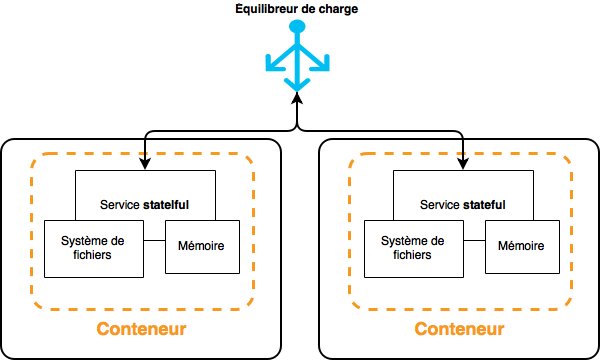
\includegraphics [scale=0.5]{chapitre4/assets/stateful}
\caption{Service non scalable}
\label{fig:non-scalable}
\end{figure}

\begin{figure}[H]
\centering
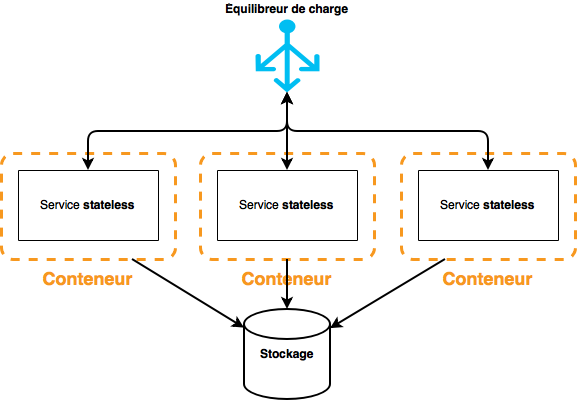
\includegraphics [scale=0.5]{chapitre4/assets/stateless}
\caption{Service scalable}
\label{fig:scalable}
\end{figure}


\section{Architecture}

\begin{figure}[H]
\centering
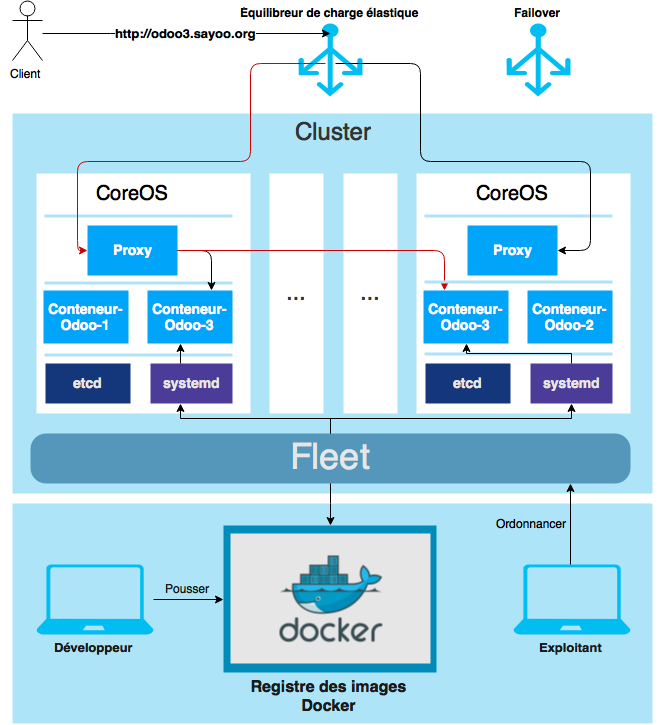
\includegraphics [scale=0.7]{chapitre4/assets/architecture}
\caption{Achitecture de la solution}
\label{fig:}
\end{figure}

L'architecture est très simplifiée car on a fait abstraction du comportement de plusieurs composants Fleet-etcd-Systemd


Il y a trois composants

-Client

-Développeur

-


L'idée c'est que une application doit être capable d'envoyer les réponses de façon consistente à partir de n'importe instance éxécutant l'application.


\end{onehalfspace}


\chapter*{Conclusion}
\addcontentsline{toc}{chapter}{Conclusion}

\begin{onehalfspace}
\initial
Notre stage de fin d'études consistait à mettre en œuvre une architecture Cloud basée sur des conteneurs. Le but de ce projet est de faciliter et simplifier aux développeurs de \emph{Sayoo} le développement, la personnalisation de nouveaux modules \emph{Odoo} (Open ERP), et faciliter le processus de déploiement continue.
\newline
\newline
Certes, c'est \emph{Odoo} qui a poussé à avoir recours au Cloud, mais la solution réalisée est conçu de façon général pour la provision des \acrshort{saas} légers (containérisés). Toutefois, elle n'est pas complète. En effet, Nous aimerions ajouter un service de mesure et de facturation ainsi que d'améliorer le processus de scalabilité et de l'automatiser.
\newline
\newline
\noindent Par ailleurs, nous suivrons avec attention le projet \emph{Flocker} qui s'intéresse à la containérisation des bases de données dans le but de perfectionner l'orchestration des applications \emph{Stateful}. Nous continuerons à surveiller le projet Deis qui intégrera Kubernetes et Mesos dans un futur proche, ce qui rendra l'architecture encore plus performante et optimale. Enfin, nous développerons des interfaces utilisateurs (UI) afin de simplifier la gestion entière de l'architecture et éviter de passer par les lignes de commandes.  	
\newline
\newline
\end{onehalfspace}

\clearpage
\printglossary[title=Glossaire, type=\acronymtype]
\clearpage
\printglossary[title=Liste des abréviations, toctitle=Liste des abréviations, type=\acronymtype]

% \chapter*{Webographie}
\begin{onehalfspace}
\theendnotes
\end{onehalfspace}
\appendix
\chapter{Odoo Sous Docker}

	Dans ce qui suit, nous allons donner une idée sur l'interface que fournit Docker pour la provision des services (conteneurs). Nous allons réalisé la mini-architecture suivante:
	
	\begin{figure}[H]
	\centering
	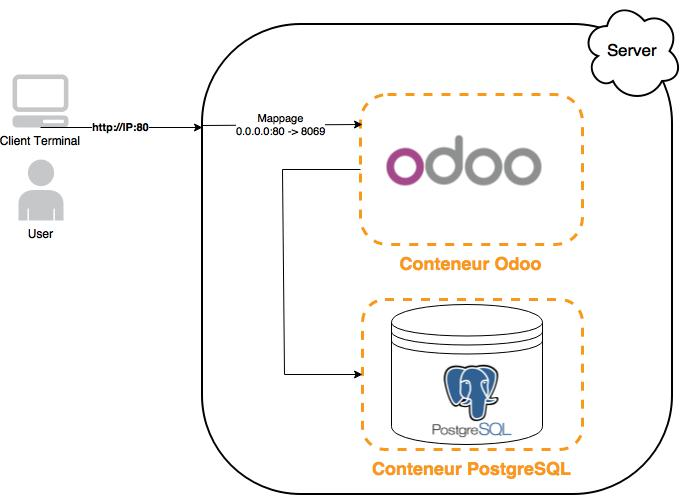
\includegraphics [scale=0.5]{biblio/odoo.jpg}
	\caption{Odoo sous Docker}
	\label{fig:}
	\end{figure}

\section*{Environnement technique}
	
	On va partir d'un serveur Ubuntu 14.04-64 bits avec Docker installé (L'installation ne sera pas détaillé), ou de préférence, un serveur CoreOS où Docker est déja inclut avec ce système d'éxploitation. A noter que Docker nécéssite un linux 64 bits avec un noyau >= 3.8.


\section*{Installation de PostgreSQL}

	Odoo a besoin d'un serveur de base de donnée PostgreSQL, la commande suivante permet de l'installer:

	\begin{lstlisting}[caption=Installation de PostgreSQL]
		$ docker run -d -e POSTGRES_USER=odoo -e POSTGRES_PASSWORD=odoo --name db postgres
	\end{lstlisting}




\section*{Installation d'Odoo}

	L'installation d'Odoo se fait grâce à la commande suivante:
	\begin{lstlisting}[language=bash,caption=Installation d'Odoo]
		$ docker run -p 80:8069 --name odoo --link db:db -t odoo
	\end{lstlisting}

	En quelques secondes, on pu lancer le service Odoo prêt à être utilisé, personnalisé, et éventuellement porté vers un autre serveur. Pour accéder au service il suffit de taper dans le navigateur:

	\begin{lstlisting}[language=bash]
		http://IP_SERVEUR:80
	\end{lstlisting}

	




\chapter{Docker-compose}

	On va réaliser l'installation détaillé dans \emph{l'Annexe A} avec l'outil \emph{Docker-compose}. Cet outil permet de définir dans un fichier \acrshort{yaml} l'architecture de l'application. Enfin, on peut faire des manipulation (démarrage, redémarrage, arrêt) sur toute l'architecture comme si c'était un seul service.

	\begin{lstlisting}[language=bash,caption=Installation d'Odoo avec Docker-compose]
		odoo:
	  		image: odoo
		  	links:
		   		- db
		  	ports:
		   		- "80:8069"
		db:
		  	image: postgres
		  	environment:
  				- POSTGRES_USER: odoo
  				- POSTGRES_PASSWORD: odoo
	\end{lstlisting}

	\begin{lstlisting}[language=bash,caption=Lancement d'Odoo avec Docker-compose]
		$ docker-compose up -d
	\end{lstlisting}



\chapter{Douze-facteurs d'un SaaS}
\label{annexe:12factors}

Dans l'informatique moderne, le logiciel est généralement livré comme un service: appelés \acrshort{saas}. Les douze-facteurs d'un SaaS est une méthodologie pour la création d'application qui:

\begin{itemize}
	\item Réduit le temps et le coût pour les nouveaux développeurs participant au projet;
	\item offre une \textbf{portabilité maximale} entre les environnements d'exécution;
	\item Sont appropriées pour le \textbf{déploiement} sur les \textbf{plates-formes de cloud} modernes, éliminant ainsi la nécessité de serveurs et d'administration de systèmes;
	\item \textbf{Réduit la divergence} entre le développement et la production, permettant un déploiement continu;
	\item peut \textbf{monter en charge} sans toucher aux outils, à l'architecture, ou à les pratiques de développement.
\end{itemize}


La méthodologie des douze-facteurs synthétise l'éxpérience de l'équipe de Heroku, un des tout premiers services cloud \cite{12-factors}. Elles peut être appliquée à des applications écrites dans n'importe quel langage de programmation, et qui sont combinées à n'importe quel services (base de données, file d'attente, mémoire cache, etc.).


\section*{code source}

Le code source de l'application doit être unique mis et suivi depuis un système de contrôle de version comme Git.

\section*{Dépendances}

La plupart des langages de programmation un sytème de gestion de dépendances. Ainsi, une application doit déclarer explicitement et isoler les dépendances. Un SaaS robuste ne repose jamais sur l'éxistence implicite des dépendances. 

\section*{Configuration}

Les variables de configurations peuvent varier entre les environnements (développement, test, production, etc). Ces variables ne doivent jamais être stockées dans des constantes à l'intérieur du code. Une bonne pratique c'est les stocker dans des variables d'environnement.

\section*{Services de support}

Traiter tous les services de support (base de données, file d'attente, serveur \acrshort{smtp}, etc.)  comme des ressources liées.

\section*{Build, release, run}

Pour déployer une application, il faut passer par trois étapes:
\begin{itemize}
	\item build: transformer le code source en exécutable;
	\item release: combiner l'exécutable avec les configurations;
	\item run: lancer les processus dans l'environnement d'exécution .
\end{itemize}


\section*{Processus}

Les processus d'une application doivent être \textbf{sans état} (stateless). Les données persistentes doivent être stockées dans une base de donnée.

\section*{Attachement de port}

Chaque service doit être exporté via un port.

\section*{Concurrence}

Les processus d'une application ne doivent jamais lancés comme un démon. Au lieu de cela,il faut compter sur le gestionnaire de processus du système d'exploitation (systemd, init.d, upstart, etc.).

\section*{Jetable}

Les processus d'une application sont jetables, ils peuvent être stoppés ou démarrés à n'importe quel moment rapidement et sans causer de problèmes.

\section*{Parité Dev/Prod}

Il faut garder tous les environnements (développement, test, production, etc) similaires.

\section*{Messages logs}

Les messages logs sont très importants, il faut les traiter comme des flux d'événements.

\section*{Processus admin}

Les taches d'administration doivent être exécutés dans un unique processus avec un environnement identique à celui du processus principal.


\chapter{Fournisseurs du Cloud}


\newpage
\end{document}